\section{Motivation}


\begin{figure}[!htbp]\captionsetup[subfigure]{font=small}
\centering
\subcaptionbox{Baseline PyTorch Approach}
[\linewidth]{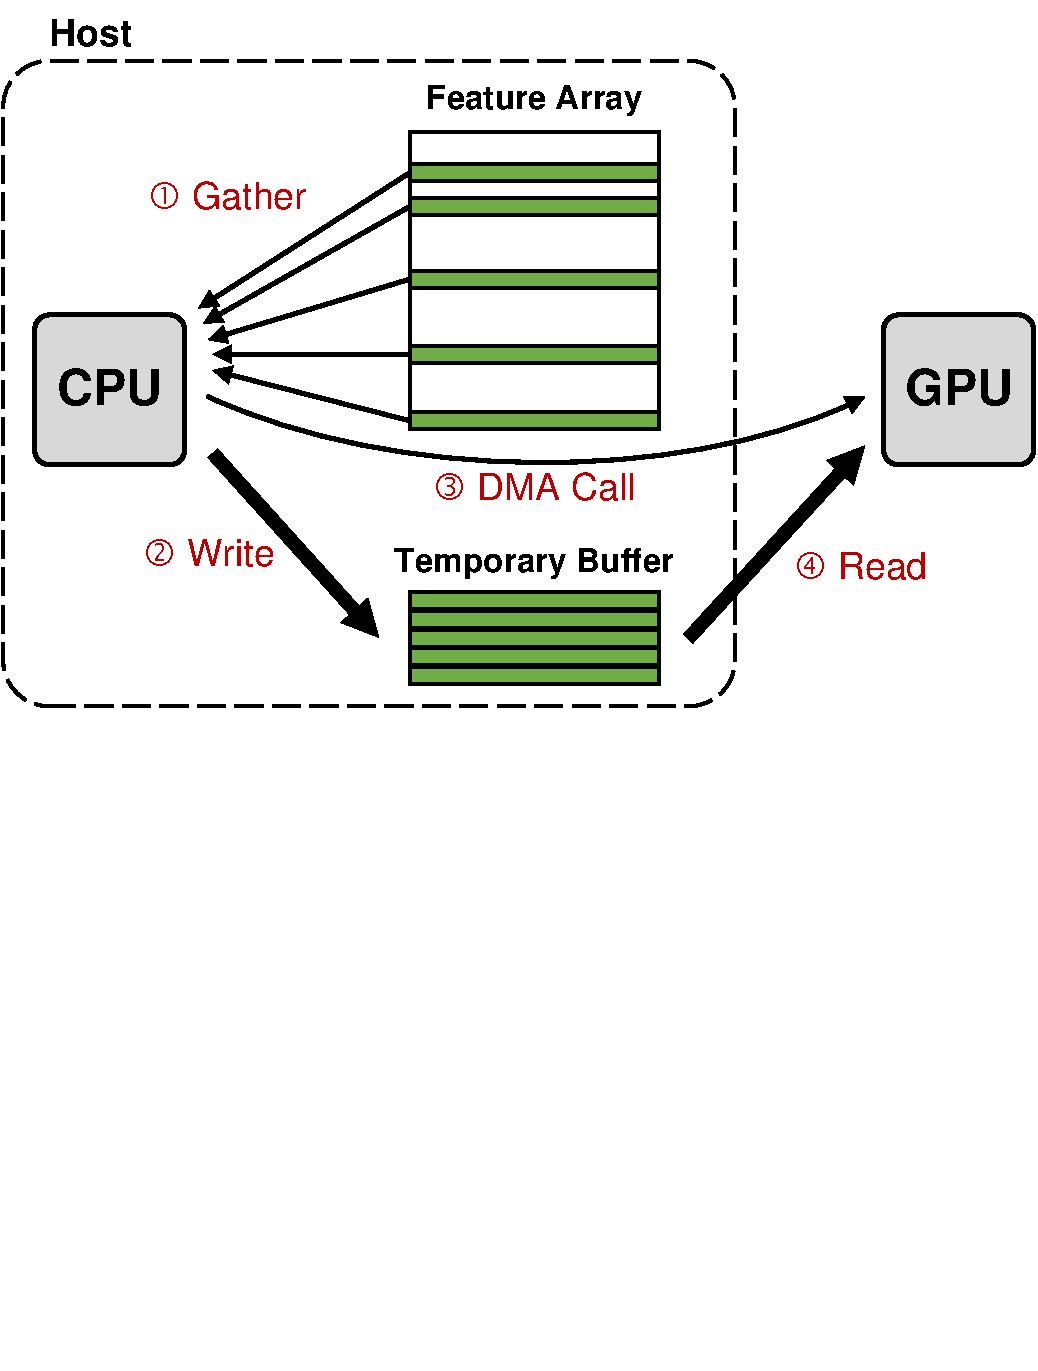
\includegraphics[scale=0.55]{figures/PyDArXiv/design_comparison_baseline.pdf}}
\subcaptionbox{PyTorch-Direct Approach}
[\linewidth]{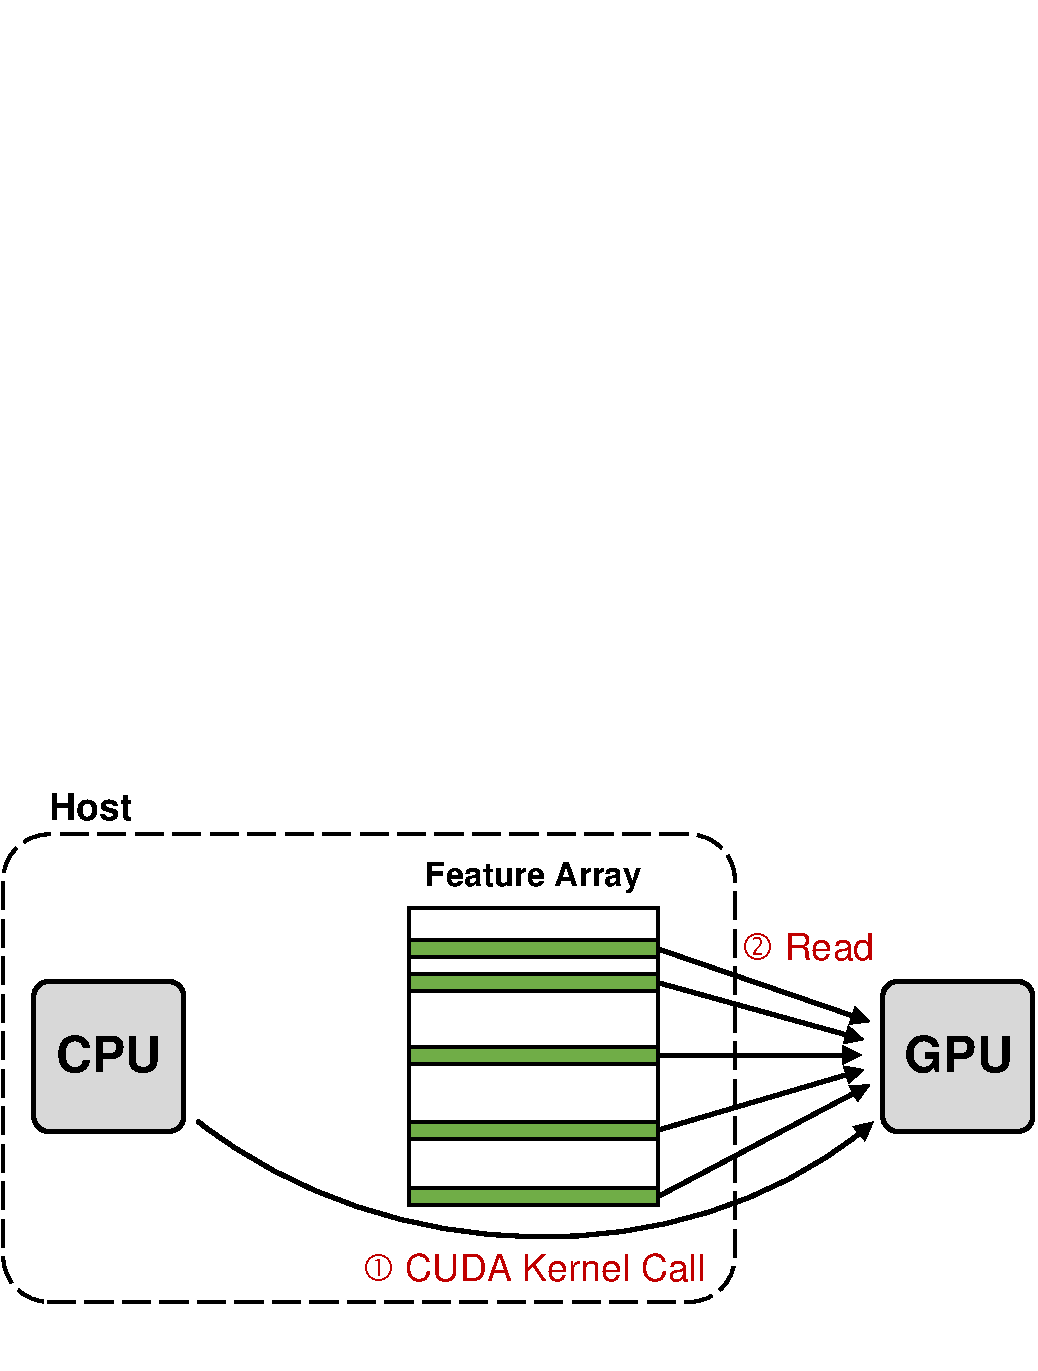
\includegraphics[scale=0.55]{figures/PyDArXiv/design_comparison_pytorch_direct.pdf}}
\caption{\label{fig:design_comparison} (a) High-level depiction of data transfer mechanism in current PyTorch implementation. (b) Simplified data transfer mechanism in PyTorch-Direct with direct access.}
\end{figure}




In current implementations of deep learning frameworks, the host-to-GPU data loading process is CPU-centric.
When data that needs to be processed by the GPU is scattered in host memory, it is the CPU's responsibility to gather the data fragments before calling a DMA.  Figure~\ref{fig:design_comparison}(a) shows the four main steps of this CPU-centric approach. The CPU first reads (gathers) the features, i.e., relevant rows of the Feature Array in this example, into its cache (\textcircled{1}),
it then writes them into consecutive locations in a temporary buffer (\textcircled{2}) 
before it calls a data copy function to set up a DMA operation (\textcircled{3}) 
and finally, the DMA hardware on the GPU reads the data from the temporary buffer in host memory into a corresponding buffer in the GPU memory (\textcircled{4}).



In Figure~\ref{fig:pyd_motivation}, we show the impact of this CPU-centric data loading approach on GNN training.
As a comparison, we use AlexNet~\cite{krizhevsky2012imagenet} and ResNet-18~\cite{He2015} as CNN examples and GraphSAGE~\cite{hamilton2017inductive} and graph attention network (GAT)~\cite{attention2018graph} as GNN examples.
We use Torchvision~\cite{torchvision} for CNN training and DGL backed by PyTorch for GNN training.
While the time spent for data loading is less than 1\% of the CNN training time, it consumes 47\% and 82\% of the GNN training time for GrapSAGE and GAT, respectively.
As the vertical axis on the right of Figure~\ref{fig:pyd_motivation} shows, CPU utilization is also much higher in GNN training.
This happens partly because the data gathering part of the code is multithreaded and tries to maximize the throughput and thus minimize latency.
Additionally, multi-threading is also used to maximize the performance of graph traversal and subgraph generation during data loading.


In short, in GNN training, unlike CNN training, data loading incurs significant time and resource overheads. In PyTorch-Direct, we aim to reduce this overhead from inefficient use of CPU resources in gather operations.
We propose a GPU-centric approach to accessing data for GNN training based on the direct host-memory-access capability of modern GPUs (Figure~\ref{fig:design_comparison} (b)).
Modern GPUs have their own address translation units and can access host memory directly.
If GPUs are connected over PCIe, they can simply generate PCIe read/write I/O
requests to the host.
From the programmer's point of view, accessing host memory can be simply done by dereferencing unified memory pointers, just like dereferencing device memory pointers.

This direct access feature is different from the conventional unified virtual memory (UVM) method, which is based on page migration.
In UVM, the data transfer between the host and GPU is done in page granularity, which is at least 4 KB per page in modern computing systems.
Whenever a required page is missing from the GPU, the CPU needs to handle the page fault through a hardware interrupt service.
Since the minimum data transfer granularity is a page and the hardware interrupt service process is costly, the performance of the UVM method depends on the applications' spatial and temporal localities~\cite{uvmguide}.
When dealing with highly irregular data structures such as a graph, using UVM incurs excessive page faults and I/O amplification~\cite{10.14778/3384345.3384358,minEMOGIEfficientMemoryaccess2020,10.1145/3342195.3387537}.

In the following section, we describe our implementation of PyTorch-Direct, which enables GPU-centric data accesses for the PyTorch DNN library.
We mainly focus on PyTorch in PyTorch-Direct due to its straightforward and intuitive way of binding data to a certain physical location from the user's perspective.
However, the main idea of the GPU-centric data accessing mechanism can still be applied to other DNN frameworks, such as TensorFlow.




\begin{figure}[!htbp]
    \centering
    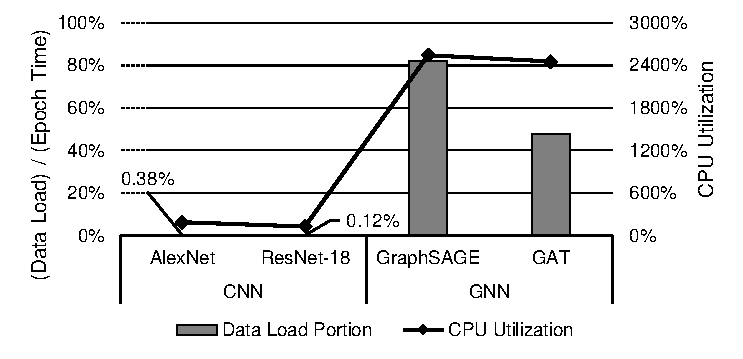
\includegraphics[width=\linewidth]{figures/PyDArXiv/motivation.pdf}
    \caption{CPU utilization and data loader time comparison between CNN and GNN training. CPU utilization can go beyond 100\% as it is multithreaded.}
    \label{fig:pyd_motivation}
\end{figure}



